
%%% Local Variables:
%%% mode: latex
%%% TeX-master: t
%%% End:

\chapter{模拟实验与性能测试}
\label{simu}
\section{引言}
前面的章节对租户网络性能的带宽保障问题进行了深入研究并提出了新的解决方案,同时设计实现了一个典型的租户应用,
为了验证所提出方案的优势,本章将对其进行实验和性能评价。

本章首先对EBG模型进行了模拟实验,之后结合DCTG系统,进行了EBG模型的性能实验。实验结果说明了,EBG模型确实
能够更加节省网络资源,同时能够解决租户需求扩张造成的问题。

\section{EBG模型性能评价实验}
\subsection{实验目的和方法}
为证明EBG模型的优势,将通过实验与其他模型进行对比,由于现有模型只有TAG能够表达应用的通信模式,所以至于TAG模型进行对比。
模拟实验将从两方面说明EBG模型的优势。

其一是从租户请求接受率上。
租户的请求并不是总能够被接受,而同样的资源,如果租户请求接受率更高,说明资源被更有效地利用了,该实验就是要
通过租户请求接受率的比较,说明EBG模型能够更好的利用数据中心资源,
从而为供应商节省成本;

其二是从租户请求扩容后,虚拟机迁移率上。
根据前面第\ref{cha:model}章的论述,租户的需求会扩展,而这会造成问题,其中主要问题就是虚拟机迁移问题。
迁移会带来严重的性能损耗,浪费大量数据中心资源,所以应当尽量避免。
这个实验通过比较迁移率,来验证EBG模型通过配置更多弹性带宽,能够有效减少迁移。

为进行模拟实验,实现了EBG模型的部署算法,并将弹性带宽为零的配置作为TAG模型(此时EBG模型等价于TAG模型)输入,进行两种模型的对比。
模拟实验在一个三层树形网络拓扑上进行,共包含2048台物理机,每个物理机包含10个虚拟机槽位。
网络上每个物理机的接入链路带宽是1Gbps,而聚合交换机和核心交换机的带宽分别为4Gbps和8Gbps。

\subsection{接受率实验}
实验中,EBG模型形如图\ref{fig:fig3.5}中的例子,因为这是最普遍的一种租户应用通信模式,
并且包含模型中的全部功能。实验随机生成大量不同组件大小,不同带宽需求的请求。
这些请求中虚拟机总数是均值为50符合指数分布的随机数,
聚合带宽保障和每台虚拟机带宽保障取不同均值的指数分布来表示不同负载的请求
(研究表明数据中心中租户虚拟机数量符合指数分布且均值为50左右,而租户的流量同样满足指数分布\cite{shieh2011sharing}),
而作为对比的TAG模型也采用均值50的指数分布随机数作为虚拟机数量,总带宽需求均值与EBG模型相同,而每台虚拟机带宽需求则是
平分总带宽需求。

实验在上一节所述网络拓扑中,生成300到500个租户请求,
通过部署算法放入网络中,计算接受的请求与总请求数的比例。
由于虚拟机槽位和网络带宽需求的限制,加上租户需求是随机生成的,
300到500个租户请求就可能将数据中心资源耗尽再也不能放入新的租户,所以实验时以连续3次部署失败作为
资源耗尽的评判标准,达成后就不再生成新的需求,而是以当前请求数来计算接受率

实验比较了不同的弹性带宽下的EBG和TAG的接受率。
$P/S$为随机生成的每虚拟机带宽保障均值与总聚合带宽保障均值的比值。
租户请求中一条边的总带宽的均值设置为1Gbps、1.5Gbps以及2Gbps。
随机生成300到500个请求后通过算法放入网络中,再计算接受率。实验结果如图\ref{fig:fig5.1}所示。

\begin{figure}[H]
  \centering
  % Requires \usepackage{graphicx}
  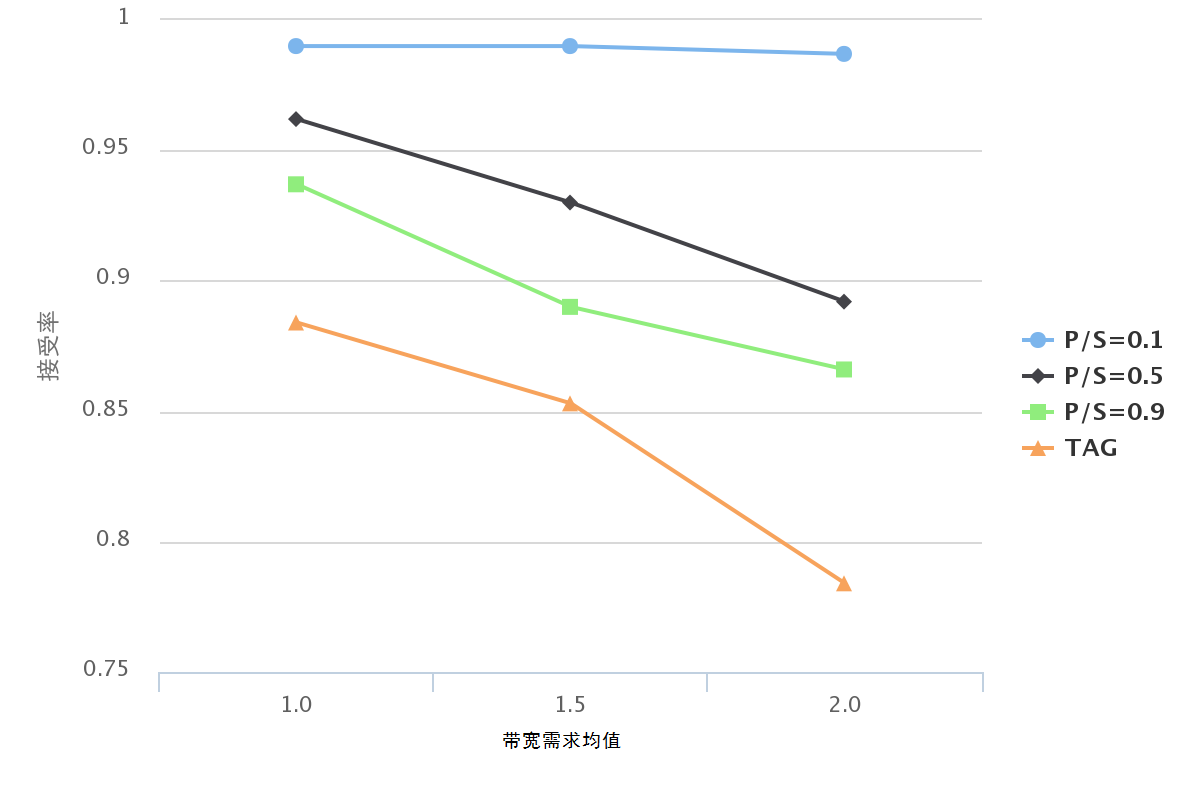
\includegraphics[width=\textwidth]{eval1}
  \caption{不同负载下EBG模型与TAG模型接受率比较}
  \label{fig:fig5.1}
\end{figure}

从图\ref{fig:fig5.1}中可以看到,随着带宽均值的提高,几种模型的接受率均有下降,
而几种模型中TAG模型的接受率最低,并且在带宽均值提高时有着明显的降低。
而EBG模型随带宽提高接受率的变化不明显,尤其当弹性带宽极高时(即$P/S$为0.1时)。
这是因为EBG模型的灵活性使得数据中心网络的资源被更有效的利用了。

\subsection{最大接受请求数实验}
另一个实验能够从侧面体现EBG的接受能力更强。实验随机生成大量请求,并进行部署,
直到连续3次分配算法失败返回,认为是数据中心网络已经接近饱和不能接受更多的租户请求,
这时比较总共接受的请求数量。这个实验目的是比较不同模型在相同的虚拟机数量和总带宽需求下,
整个数据中心网络能够接受的总请求数,能够接受更多请求的模型说明资源利用率更高。
结果如表\ref{tab:tab2}所示,其中数据是多次实验取平均值的结果,所以请求数不是整数。

\begin{table}[h]
  \centering
  \caption{不同模型最大接受请求数比较}
  \label{tab:tab2}
  \begin{tabular}{c | c c c c}
  \hline
  $P/S$ & TAG & 0.1 & 0.5 & 0.9 \\ \hline
  平均最大接受请求数 & 297.8 & 452.5 & 459.3 & 458.3 \\
  \hline
  \end{tabular}
\end{table}

从表\ref{tab:tab1}中数据可以看到,即使增加$P/S$比例,EBG能够接受的请求数量并没有受到太大影响,而由于网络拓扑中总共有20480个虚拟机槽位,每个请求的期望虚拟机数是50,所以这个最大请求数是受虚拟机槽位限制的。而TAG的接受能力却低了很多,且完全没有使用掉网络中的虚拟机槽位,可见是带宽资源限制了其接受请求。可以看到EBG模型的接受能力即使在每虚拟机带宽均值与总聚合带宽均值比值达0.9时,依然远超TAG模型,而这时不仅EBG模型请求的总带宽与TAG请求的总带宽相同,每个虚拟机的带宽保障也十分接近,EBG模型的带宽保障能力与TAG是几乎相同的。

从接受率实验中可以验证EBG模型的接受率高于TAG模型,而这正是由于弹性带宽的存在,使得EBG模型能够更好的利用数据中心的网络资源。

\subsection{租户扩容后迁移率实验}
这个实验先接受多个租户的请求,构成当前网络状态,记录下当前虚拟机的部署情况。之后随机将这些租户中的一部分的需求增加,增加其请求的虚拟机数量,之后计算旧有的虚拟机中改变位置的数量,比上虚拟机总数,得到迁移率。

实验首先在网络中部署100个虚拟机数量期望50的租户,之后按照一定比例增加虚拟机数量(在三个组件中随机选择一个),重新部署后,计算迁移的虚拟机数量与原虚拟机数量的比值。为比较TAG与EBG,租户的总带宽需求两种模型都是期望为1Gbps,而TAG的每虚拟机带宽需求按照定义由所有虚拟机平分总带宽,
结果如图\ref{fig:fig5.2}所示。

\begin{figure}[H]
  \centering
  % Requires \usepackage{graphicx}
  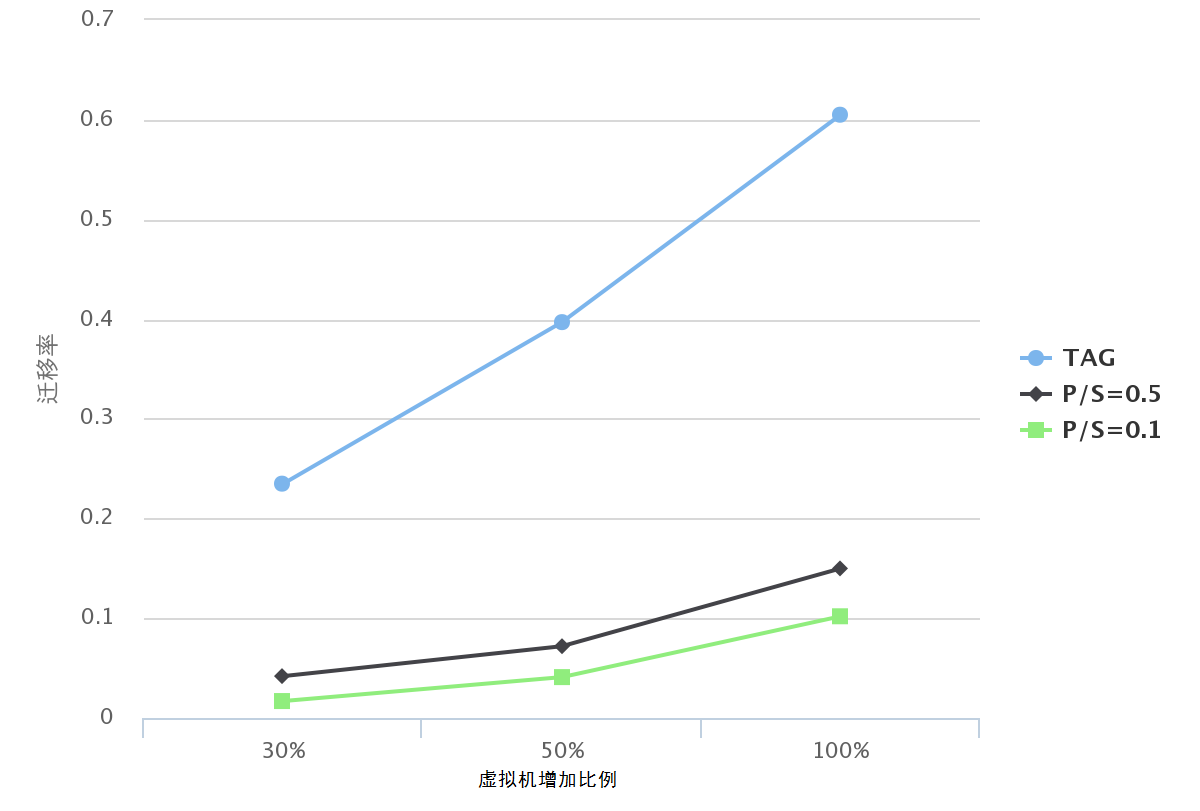
\includegraphics[width=\textwidth]{eval2}
  \caption{不同虚拟机数量增加比例下迁移率比较}
  \label{fig:fig5.2}
\end{figure}

从图中可以看到,虚拟机增加比例有30\%、50\%、100\%三种,对于EBG模型来说无论$P/S$比例是0.1还是0.5,都只有很少一部分虚拟机发生迁移。而TAG模型却有大量虚拟机迁移,在虚拟机数量增加100\% 时,甚至有60\%的原虚拟机发生迁移。

实验表明EBG模型确实能够通过充足的弹性带宽来减少发生迁移的概率,而且比起没有考虑扩容问题的TAG模型,EBG模型在这一问题上有着明显的优势。

\section{结合DCTG系统进行EBG模型性能实验}
\subsection{DCTG系统建模}
DCTG系统作为一个对网络性能十分看重的租户应用,租户带宽保障方案十分适用于这个系统。
而在各类租户带宽保障模型中,EBG模型对DCTG系统尤其适用。因为对于DCTG系统而言,只关注总带宽,而不关心每个client
的带宽,如果总带宽足够高,就能生成需要的流量,而EBG模型保障租户组件的总带宽的设计刚好符合这一点。
DCTG这样的租户应用在使用EBG模型时,能够充分享受到弹性带宽带来的优势。

要对DCTG系统使用带宽保障方案,首先需要对DCTG这一租户应用建模。使用EBG对DCTG建模如图\ref{fig:dctgmodel}。

\begin{figure}[h]
  \centering
  % Requires \usepackage{graphicx}
  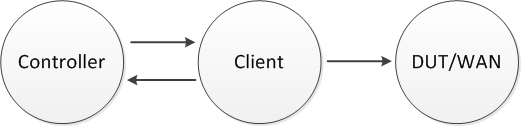
\includegraphics[scale=0.6]{DCTG}
  \caption{使用EBG对DCTG建模}
  \label{fig:dctgmodel}
\end{figure}

DCTG系统包含两个组件,controller和client,互相之间有着通信,而一般这部分的通信主要是DCTG系统的统计信息从client
汇报给controller,并不需要很大的带宽保障。另外最主要的就是从client发送出去的流量,这部分流量会发送给被测单元。
而如果DCTG测试的是云外的设备,这部分流量在云内部首先需要送到云的对外网关。所以可以看到,图中模型的最右边的组件
有可能是云内部的被测单元,也有可能是出口网关。

这个EBG模型有一个特殊之处,就是其中被测单元(或者网关)这部分并不属于租户本身,这部分并不属于租户请求,
而其在数据中心中的位置也已经确定。这样对于EBG模型的虚拟机分配算法,需要稍作改动,将这一部分看作是已经确定好位置的
组件,无需进行分配,但需要考虑其带宽保障。

\subsection{实验结果}
将DCTG建模后,就可以进行实验。实验同样对EBG模型和TAG模型,比较其接受率和迁移率。
实验中controller的组件平均大小为10VM,client的大小为平均30VM,被测单位大小平均为10VM,
随机在云中选择位置。Controller与client间的平均带宽均为500,client发送到被测单元的带宽取不同的均值来进行对比。
结果如图\ref{fig:dctgeval1}。

\begin{figure}[H]
  \centering
  % Requires \usepackage{graphicx}
  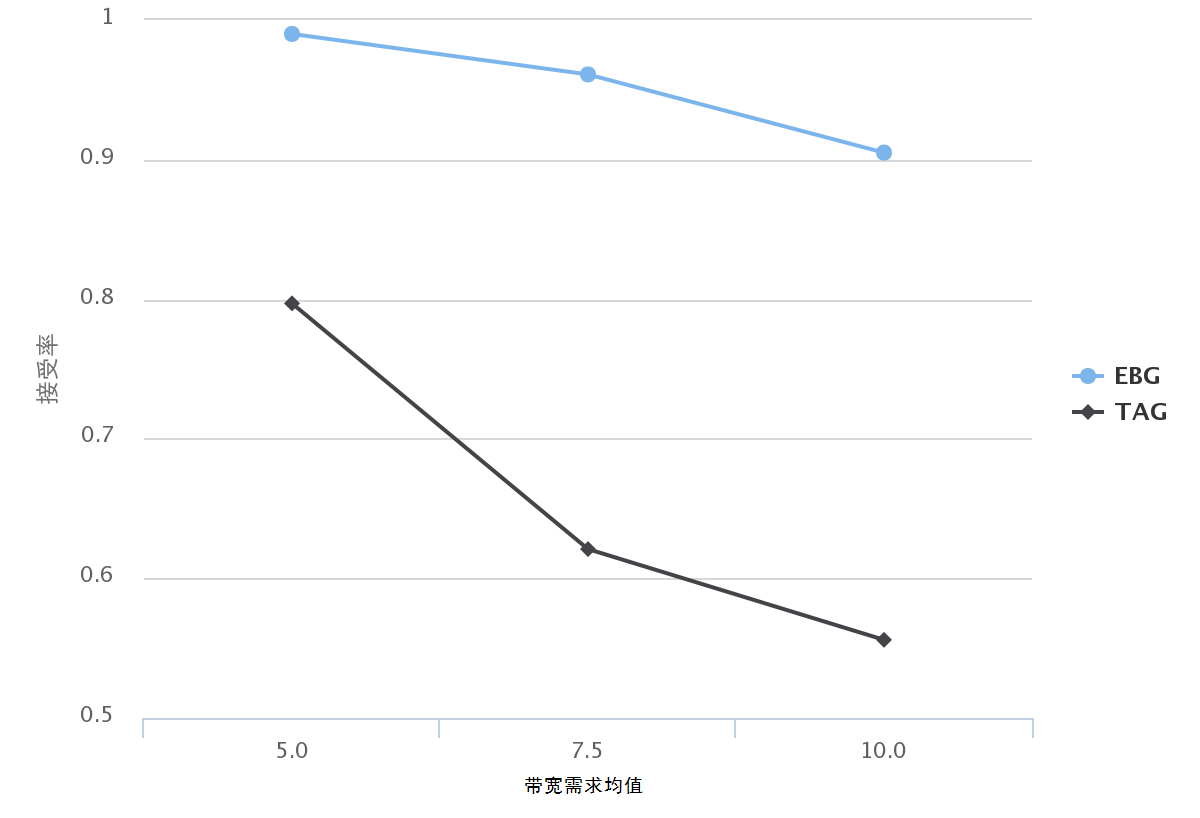
\includegraphics[width=\textwidth]{dctgeval1}
  \caption{DCTG建模的接受率比较}
  \label{fig:dctgeval1}
\end{figure}

图中可以看到,对于DCTG使用EBG和TAG分别建模,其接受率差异明显,EBG依靠弹性带宽几乎达到了100\%的接受率,
而少数不能接受的租户请求是因为被测单元的带宽限制。而TAG则接受率明显比EBG低。

\begin{figure}[H]
  \centering
  % Requires \usepackage{graphicx}
  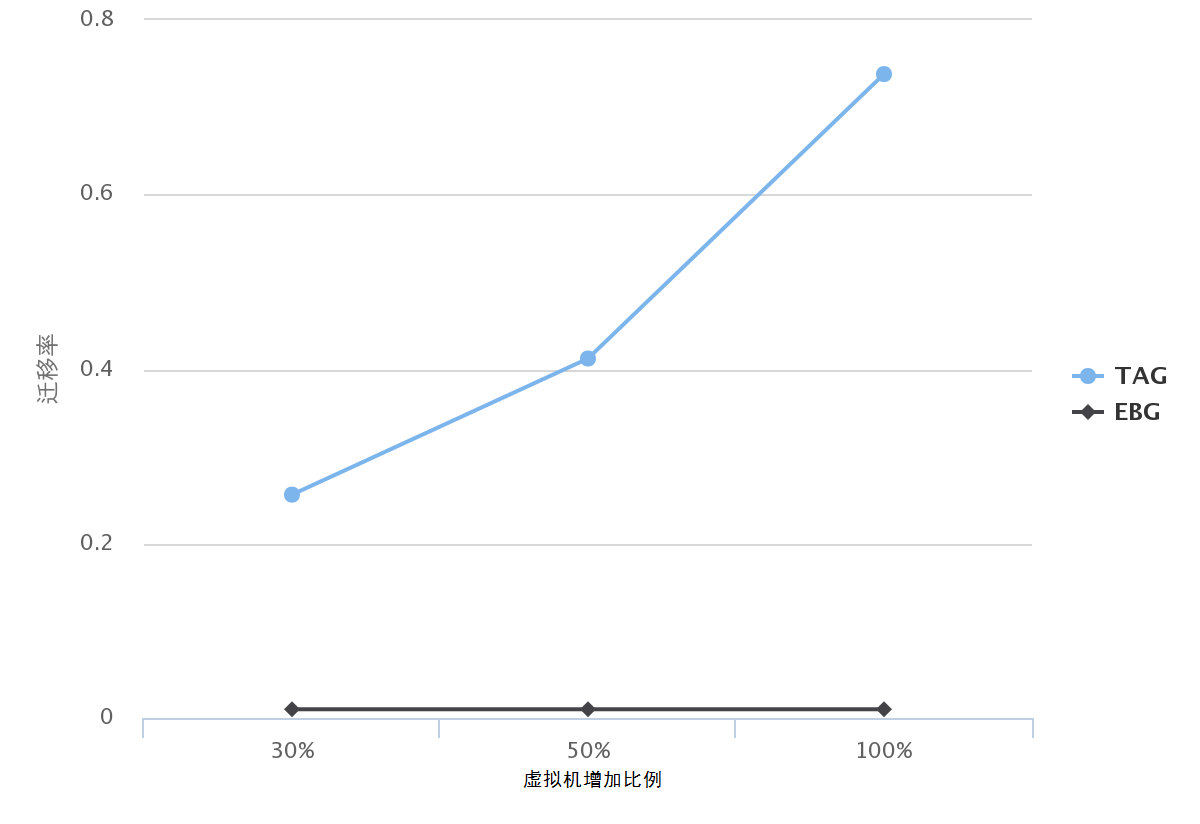
\includegraphics[width=\textwidth]{dctgeval2}
  \caption{DCTG建模的迁移率比较}
  \label{fig:dctgeval2}
\end{figure}

迁移率实验结果如图\ref{fig:dctgeval2}。EBG模型几乎不发生迁移,而TAG模型仍然发生大量迁移。
而这正是因为EBG模型建模DCTG系统,并没有每台虚拟机的带宽限制,拥有充足的弹性带宽。

由于DCTG应用的性质,使用EBG建模明显更具优势,而EBG模型的灵活性在DCTG这一类不需要每台虚拟机带宽
限制的应用上有了最大的体现。实验结果完全说明,EBG模型拥有TAG模型所不具备的灵活性,同时能够解决
租户需求变化带来的迁移问题。

\section{小结}
本章通过模拟实验,说明了EBG模型的性能优势。通过接受率的对比,说明了EBG模型能够更加有效的利用
数据中心的资源;而通过迁移率的比较,说明了EBG模型能够有效解决这一问题。同时将DCTG系统建模,进行了
实验并进一步说明了EBG模型的优势。

EBG模型的核心是弹性带宽和灵活性,通过灵活性,将租户带宽保障这一问题得以有效的解决。
